

	\begin{figure}[h!]
		\centering
		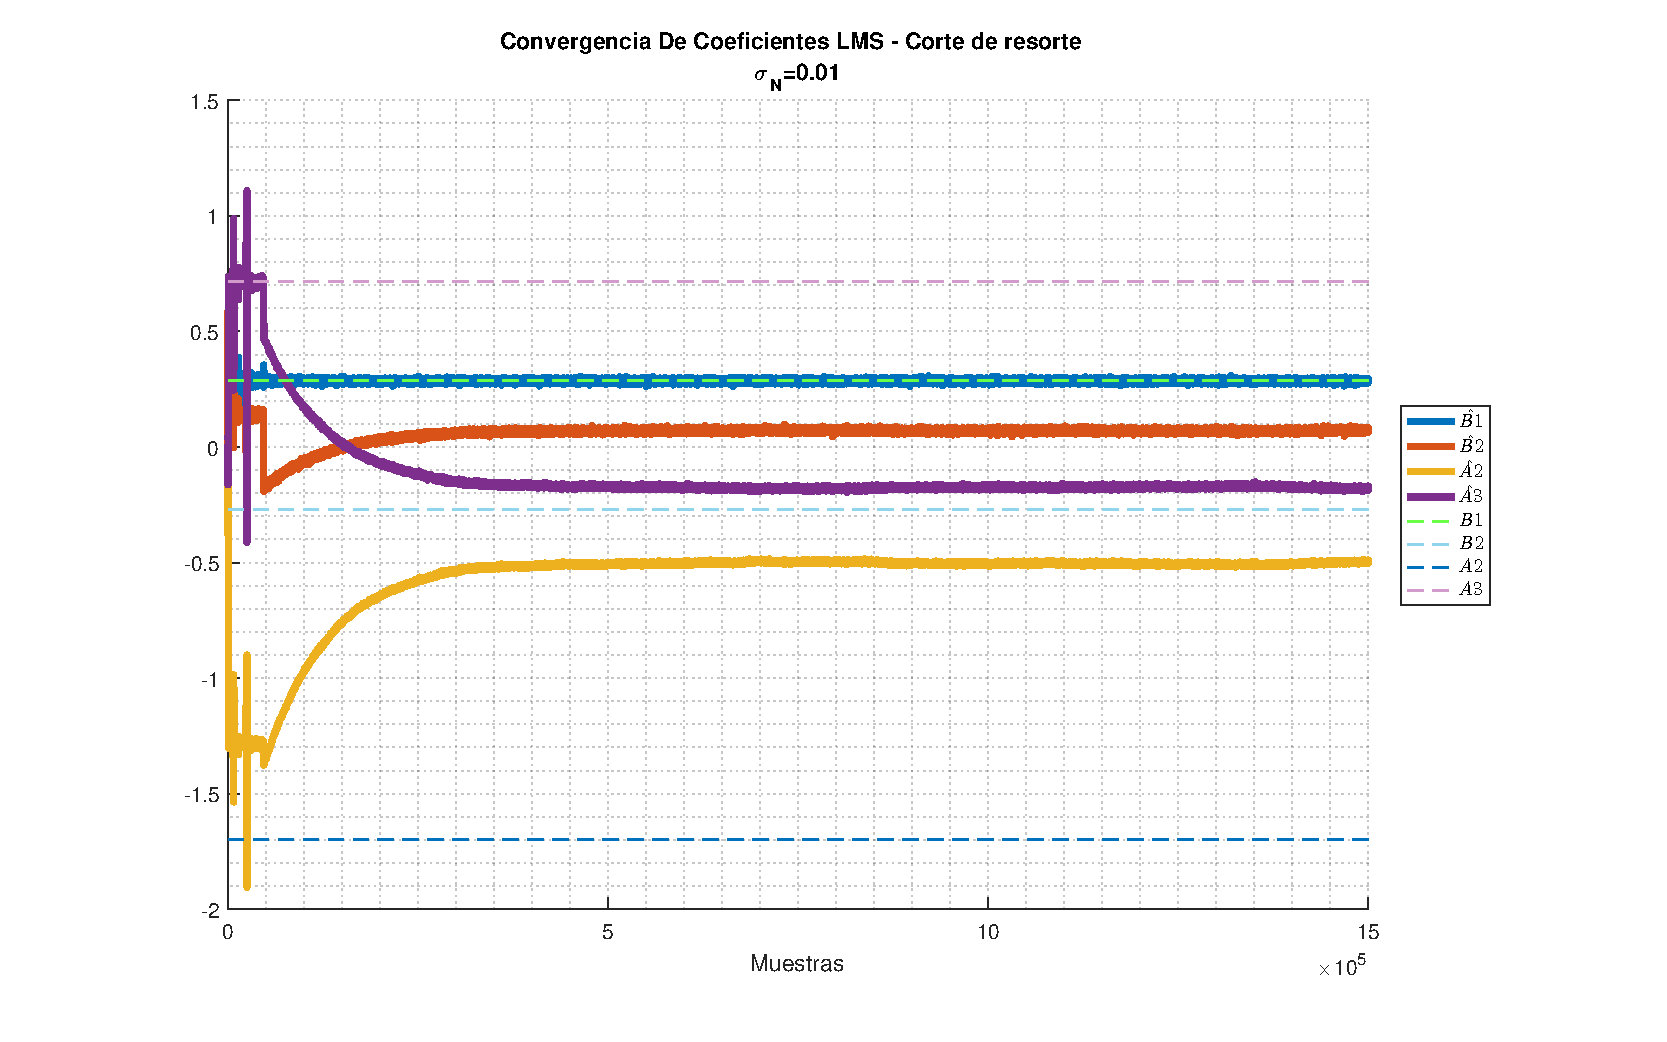
\includegraphics[width=0.8\textwidth]{graf_ej4.pdf}
		\caption{Convergencia de los parámetros si se corta el resorte con $\sigma_N = \SI{.01}{\m}$.}
		\label{fig:ej4}
	\end{figure}

	En la presente Sección se analiza el caso en que se corta el resorte en el medio de la simulación, es decir que la constante $k$ se anula. Las variaciones de los coeficientes se presentan las Figuras \ref{fig:ej4} y \ref{fig:ej4bis}. 
	Se propone que $k\neq0$ en particular \num{.1} porque de lo contrario la convergencia es muy lenta. Si se supone que el error es del orden de \SI{.01}{\m} se ve en la Figura \ref{fig:ej4} que los coeficientes no convergen a los valores correctos. En cambio si se supone incertidumbres del orden de \SI{0.001}{\m} converge mejor aunque lentamente (\ref{fig:ej4bis}). 

	\begin{figure}[h!]
		\centering
		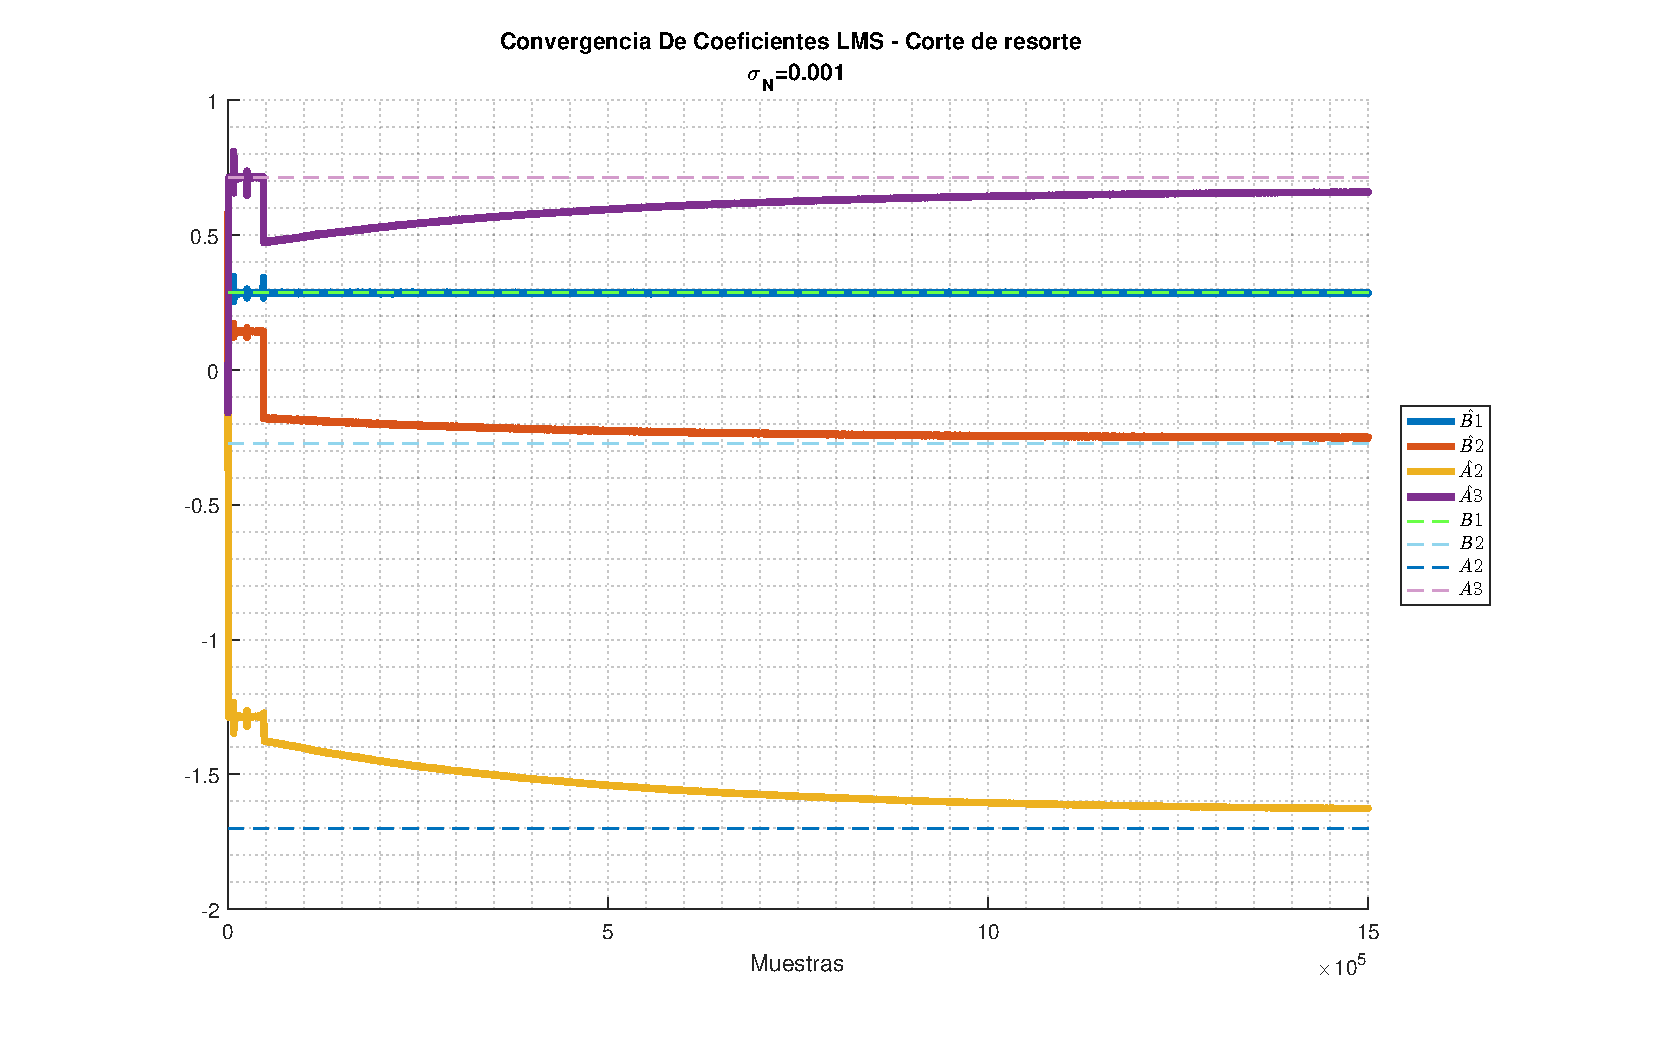
\includegraphics[width=0.8\textwidth]{graf_ej4bis.pdf}
		\caption{Convergencia de los parámetros si se corta el resorte con $\sigma_N = \SI{.001}{\m}$.}
		\label{fig:ej4bis}
	\end{figure}


	
		\begin{table}[h!]
			\centering
			\begin{tabular}{cccc}
				\toprule
				&$m$ (fija)	& $k$	& $b$\\
				\midrule
				$\sigma_N=\num{.01}$&5&$\num{2.4955}$&$\num{2.0053}$\\
				$\sigma_N=\num{.001}$&5&$\num{0.2455}$&$\num{2.0007}$\\
				\bottomrule
			\end{tabular}
		\end{table}

		La estimación de $k$ difiere mucho del valor real cuando el ruido es alto. Este resultado coincide con la mala estimación de los coeficientes de la Figura \ref{fig:ej4}. Del mismo modo se ratifica la buena estimación cuando el ruido es bajo, obteniendose $k=\num{0.2}$ y una mejor convergencia en la Figura \ref{fig:ej4bis}.
